\documentclass[pdf]{beamer}
\mode<presentation>{
	\usetheme{Ilmenau}
	
}
\usecolortheme{beaver}
%\usepackage[UTF8,indent]{ctexcap}%中文
\usepackage{amssymb}
\usepackage{amsmath}
\usepackage{amsfonts}
%\usepackage{graphicx}
\usepackage{amsthm}
\usepackage{indentfirst}
\usepackage{enumerate}
\usepackage{extpfeil}
\usepackage{tikz-cd}
\usepackage{longtable}

\usetikzlibrary {calc,positioning,shapes.misc,graphs,decorations.pathreplacing}
\usefonttheme[onlymath]{serif}

\numberwithin{equation}{section}

\theoremstyle{plain}
\newtheorem{proposition}[theorem]{Proposition}
\newtheorem{claim}[theorem]{Claim}
\newtheorem{defn}[theorem]{Definition}
\newtheorem{eg}[theorem]{Example}

\theoremstyle{plain}
\newtheorem{exercise}{Exercise}[section]


\theoremstyle{remark}
\newtheorem{remark}[theorem]{Remark}
\newtheorem{remarks}{Remarks}
\newtheorem{ex}[theorem]{Exercise}
\newtheorem{question}[theorem]{Questions}
\newtheorem{short}{ }

\newcommand*{\thick}[1]{\text{\boldmath$#1$}}
\newcommand*{\cir}[1]{\;$\ding{19#1}$\;}%临时使用
\newcommand*{\norm}[1]{\lVert#1\rVert}

\DeclareMathOperator{\supp}{supp}
\DeclareMathOperator{\dist}{dist}
\DeclareMathOperator{\vol}{vol}
\DeclareMathOperator{\diag}{diag}
\DeclareMathOperator{\tr}{tr}
\DeclareMathOperator{\Proj}{\operatorname{Proj}}
\DeclareMathOperator{\Aut}{\operatorname{Aut}}
\DeclareMathOperator{\Img}{\operatorname{Im}}
\newcommand*{\bigchi}{\mbox{\Large$\chi$}}% big chi
\setlength{\parindent}{1em}
\newcommand{\character}[2]{\left[\begin{array}{c}{#1} \\ {#2}\end{array}\right]}
\newcommand{\normalcharacter}{\character{\epsilon}{\epsilon'}}

\setbeamertemplate{caption}[numbered]
% 设置图形文件的搜索路径
\graphicspath{{figures/}}
\title{Dessin d'enfant: an Introduction}
\author{Xiaoxiang Zhou}
\institute[USTC]{University of Science and Technology of China}
\date{\today}
\tikzset{
	invisible/.style={opacity=0,text opacity=0},
	visible on/.style={alt=#1{}{invisible}},
	alt/.code args={<#1>#2#3}{%
		\alt<#1>{\pgfkeysalso{#2}}{\pgfkeysalso{#3}} % \pgfkeysalso doesn't change the path
	},
}
\setbeamercolor{section number projected}{fg=white!90!blue, bg=red!90!black}
\setbeamercolor{block body}{fg=black,bg=gray!10}
\setbeamercolor{block title}{fg=white, bg=red!64!black}


\setbeamertemplate{headline}{
	\begin{beamercolorbox}[wd=\paperwidth,ht=2.5ex,dp=1.125ex]{section in head/foot}%
		\hspace{3ex}{\insertsectionhead}
	\end{beamercolorbox}
	%	\begin{beamercolorbox}[ht=2.5ex,dp=1.125ex,leftskip=.3cm,rightskip=.3cm plus1fil]{subsection in head/foot}
	%		\usebeamerfont{subsection in head/foot}\insertsubsectionhead
	%\end{beamercolorbox}
}%删除点
\begin{document}
\begin{frame}
	\titlepage
\end{frame}
\begin{frame}
\begin{abstract}
	In this talk, we will talk about \textbf{the relation between Belyi map and dessin d'enfant}, and than extract imformations from the dessin.
	
	Contents: section 4.1-4.3 and some examples from section 4.6.
\end{abstract}
\end{frame}
\begin{frame}{Contents}
\tableofcontents
\end{frame}


\begin{frame}{Introduction}
 Last time, we talked about the Belyi's Theorem:
\begin{theorem}[Thm 3.1]
	Let $S$ be a cpt RS, then $S$ is defined over $\bar{\mathbb{Q}}$ iff $S$ admits a Belyi fct.
\end{theorem}

This time, we talked a specific Belyi fct (ramified at $0,1,\infty$), and

\begin{itemize}
	\item combine it with a kind of \textbf{special graph} (on $S$);
	\item extract information from this graph.
\end{itemize}
\end{frame}
\section{Belyi fct}
\begin{frame}{Contents}
\tableofcontents[currentsection]
\end{frame}
\begin{frame}{Black box}
	\begin{center}
		\fbox{\textbf{Prop 3.34:} Belyi fcts are defined over $\bar{\mathbb{Q}}$.}
		%%%%更逼真的盒子
	\end{center}
\begin{remark}
	We can talk about the Galois group 
	\begin{center}
		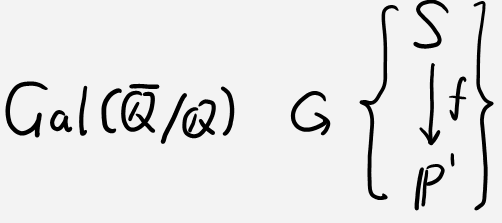
\includegraphics[width=0.3\textwidth]{figures/Galaction.png}
	\end{center}
	%%%%%%%%画图
\end{remark}
\end{frame}
\begin{frame}{Example}

		When $S=\mathbb{P}^1$, then an Belyi fct $f(z)$ (not constant since we consider fct ramified on three points) is an rational fct with \textbf{coefficient in $\bar{\mathbf{Q}}$} such that $f$ maps any zero or pole of $f'(z)$ to $0,1,\infty$. In short,
	\begin{short}
		\begin{itemize}
			\item  $f(z) \in \bar{\mathbb{Q}}(z)$;
			\item For any $z_0$ such that $f'(z_0)=0 \text{ or } \infty$, $f(z_0)=0,1 \text{ or } \infty$.
		\end{itemize}
	\end{short}
\end{frame}
\begin{frame}
			For example,
	\begin{itemize}
		\item $f(z)=z^n$;
		\item $\displaystyle f(z)=-\frac{256}{27}z^3(z-1)$;
		\item $\displaystyle f(z)=\frac{3+i}{5}z^3(z-1)^2 \left(z-\frac{4}{25}(4+3i) \right)$;
		\item $\displaystyle f(z)=\frac{4}{27} \frac{(1-z+z^2)^3}{z^2(z-1)^2}$;
		\item $\displaystyle f(z)=C\frac{z^4 (z-1)^2}{z-\frac{11+2\sqrt{10}}{18}}, \qquad C \approx -9.55063$.
	\end{itemize}

\end{frame}
%%%%%%%%%%%%%%%%%%%%%%%%%%%%%%%%%%%%%%%%%%%%%%%%%%%%%%%%%%%%%%%%%%%%%%%%%%%%%%%%%%%%%%%%%%%%%%%
\section{What is a dessin d'enfants? / Quel est un dessin d'enfants ?}
\begin{frame}{Contents}
\tableofcontents[currentsection]
\end{frame}
\begin{frame}{Better question}
	We postponed the abstract definition of the dessin d'enfant. 
	
	A better question: How to draw a dessin d'enfants from a Belyi fct?
	\only<2>{	\begin{center}
			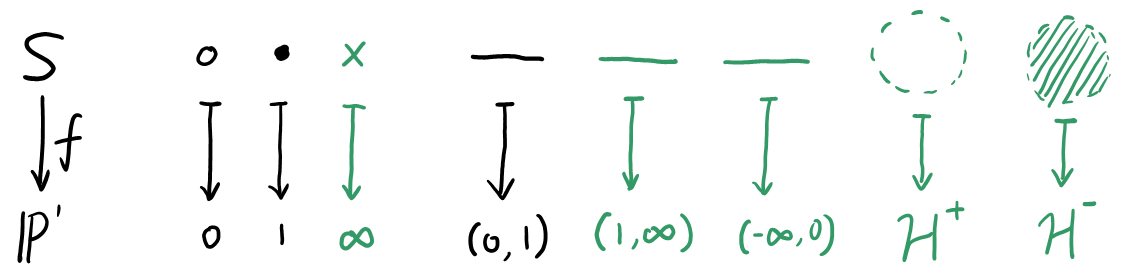
\includegraphics[width=0.8\textwidth]{figures/drawdes.png}
	\end{center}}
\only<3>{	\begin{center}
		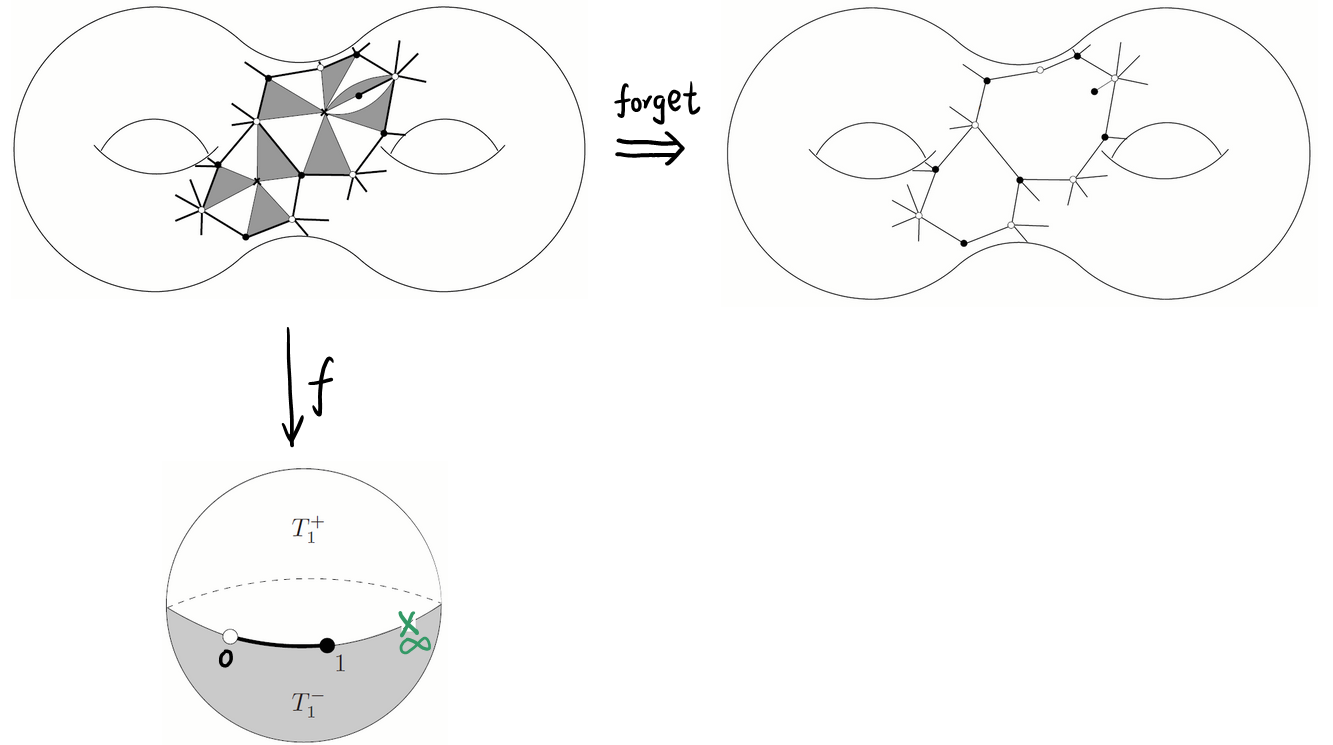
\includegraphics[width=0.8\textwidth]{figures/drawdes2.png}
\end{center}}
	
\end{frame}
\begin{frame}
	\begin{proposition}
		\begin{itemize}
			\item the graph $D$ is drawed on the RS $S$;
			\item $D$ is bicolored;\hspace{1cm}
\includegraphics[width=0.1\textwidth]{figures/des1.png}
			\item $X \smallsetminus D$ is union of finitely many topo discs;
					\begin{center}
						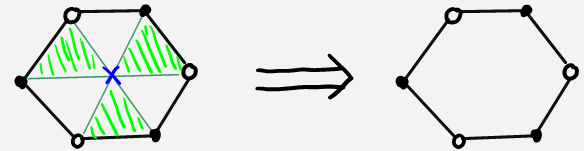
\includegraphics[width=0.5\textwidth]{figures/des2.png}
					\end{center}
			\item $D$ is connected.
		\end{itemize}
	\end{proposition}
\end{frame}
\begin{frame}{Abstract definition}
	\begin{defn}[Def 4.1]
		\textbf{A dessin d'enfant}, or simply \textbf{a dessin}, is a pair
		$(X, \mathcal{D})$ where $X$ is an \textbf{oriented} compact topological surface, and
		$\mathcal{D} \subset X$ is a finite graph such that: 
		\begin{itemize}
			\item  $\mathcal{D}$ is \textbf{connected}.
			\item  $\mathcal{D}$ is \textbf{bicoloured}, i.e. the vertices have been given either white or black colour and vertices connected by an edge have different colours.
			\item  $X \smallsetminus \mathcal{D}$ is the union of finitely many \textbf{topological discs}, which we call \textbf{faces} of  $\mathcal{D}$.
		\end{itemize}
	\end{defn}
\end{frame}
\begin{frame}[fragile]{Pictures}
\begin{figure}[th]
	\begin{minipage}[b]{.35\textwidth}
		\centering
		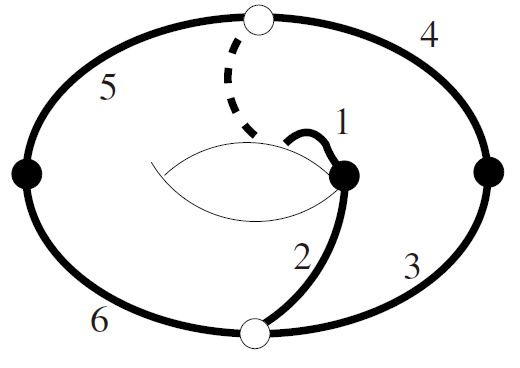
\includegraphics[height=.3\textheight]{figures/Fig4-3.png}
	\end{minipage}
	\begin{minipage}[b]{.4\textwidth}
	\centering
	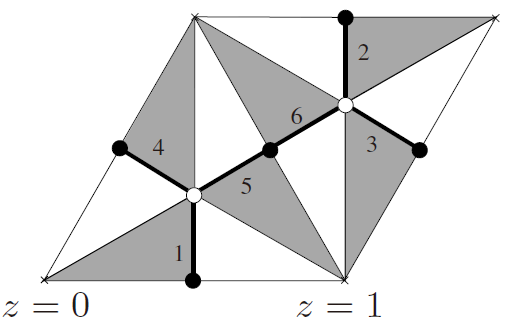
\includegraphics[height=.3\textheight]{figures/Fig4-6.png}
\end{minipage}
\end{figure}
	\begin{figure}[th]
	\begin{minipage}[b]{\textwidth}
		\centering
		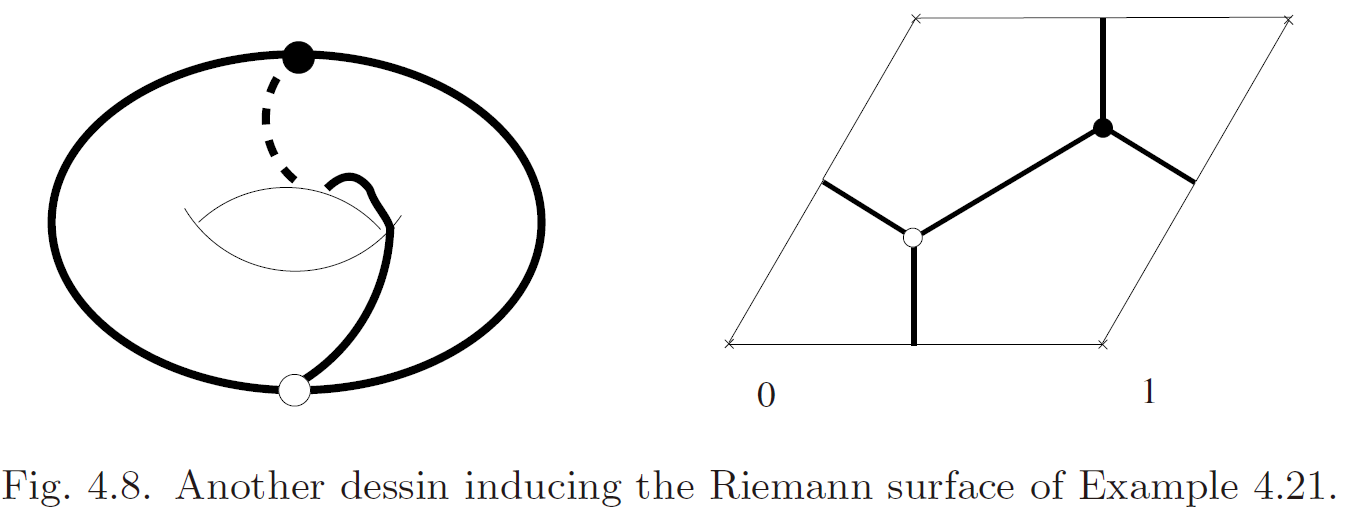
\includegraphics[height=.33\textheight]{figures/Fig4-8.png}
	\end{minipage}
\end{figure}
\end{frame}
\begin{frame}[fragile]{Pictures}
	\begin{figure}[th]
	\begin{minipage}[b]{\textwidth}
		\centering
		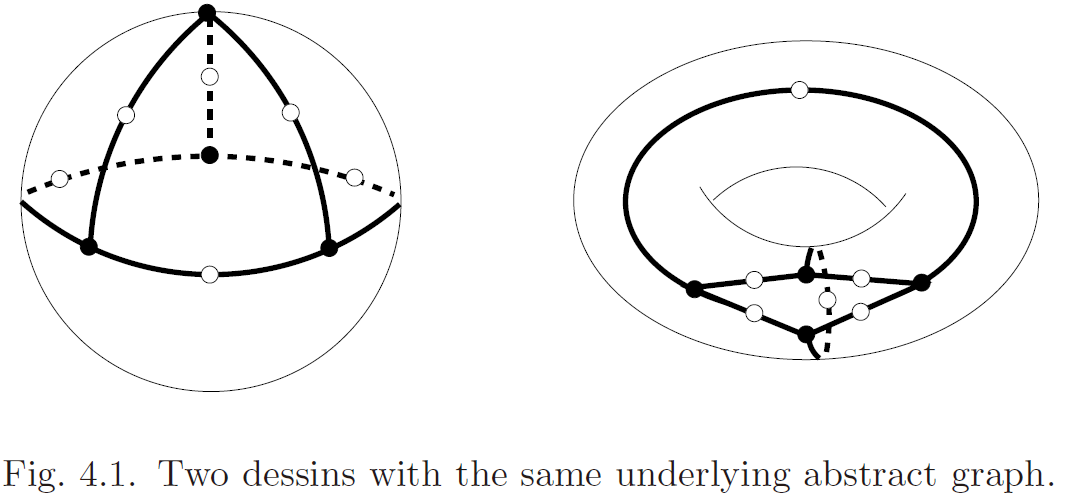
\includegraphics[width=0.72\textwidth]{figures/Fig4-1.png}
	\end{minipage}
\end{figure}

\end{frame}
\begin{frame}[fragile]{Pictures}
\begin{figure}[th]
	\begin{minipage}[b]{\textwidth}
		\centering
		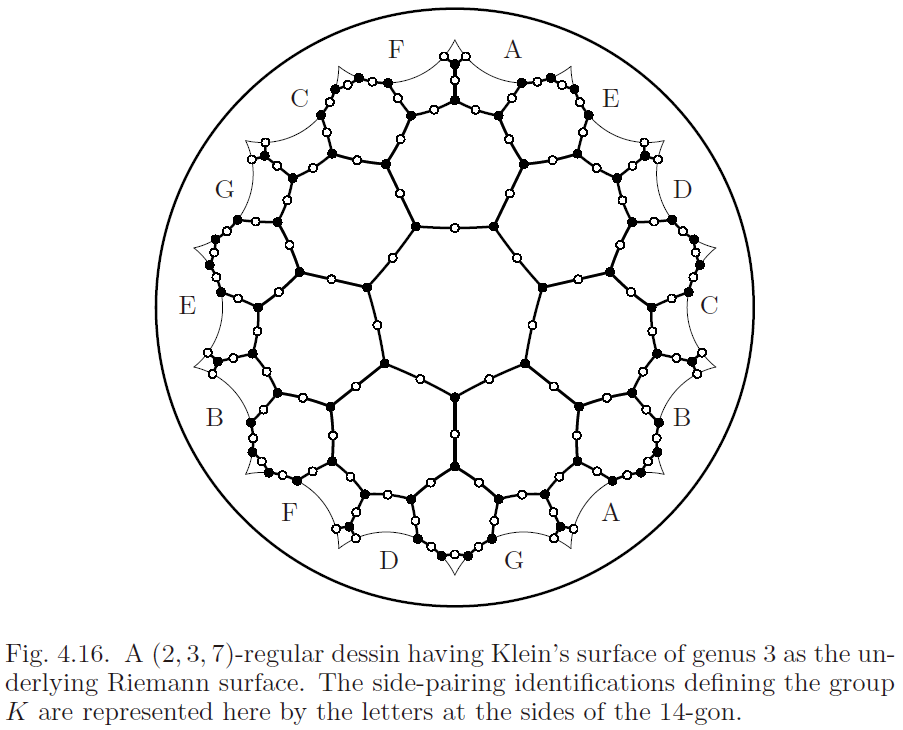
\includegraphics[width=0.72\textwidth]{figures/Fig4-16.png}
	\end{minipage}
\end{figure}
\end{frame}
\begin{frame}[fragile]{Pictures}
\begin{figure}[th]
	\begin{minipage}[b]{.4\textwidth}
		\centering
		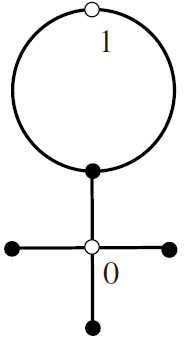
\includegraphics[width=0.4\textwidth]{figures/Fig4-32-1.png}
	\end{minipage}
	\begin{minipage}[b]{.4\textwidth}
	\centering
	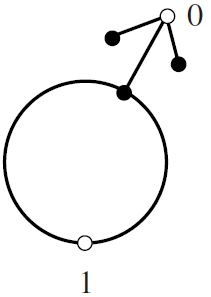
\includegraphics[width=0.5\textwidth]{figures/Fig4-32-2.png}
\end{minipage}
\end{figure}
\end{frame}
\begin{frame}[fragile]{Pictures}
\begin{figure}[th]
	\begin{minipage}[b]{\textwidth}
		\centering
		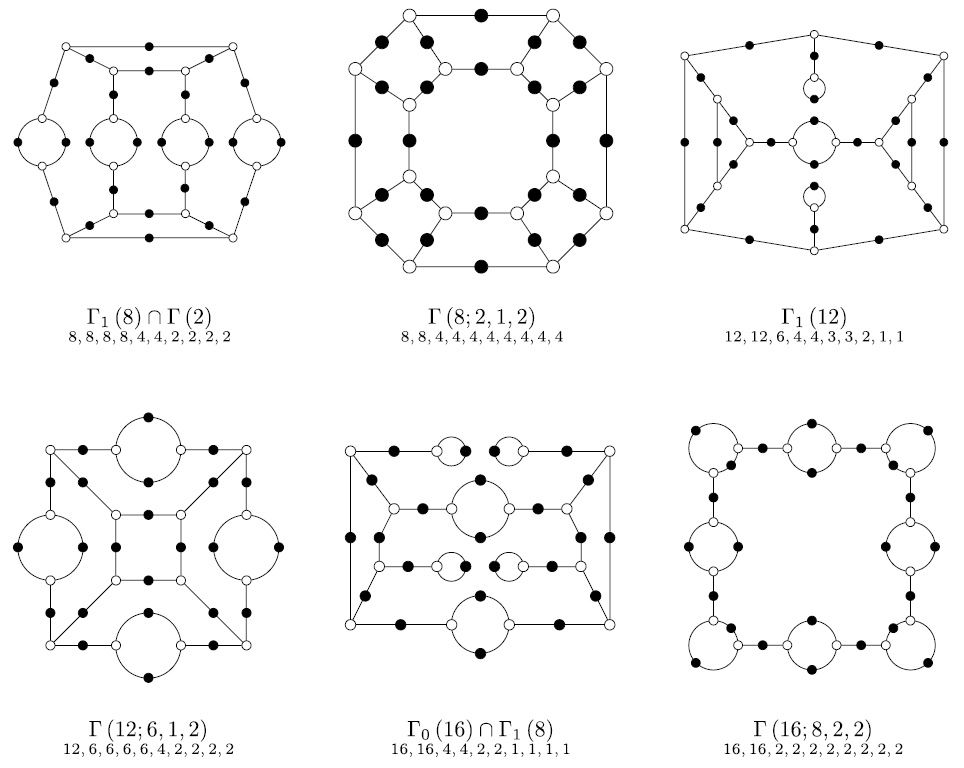
\includegraphics[width=0.8\textwidth]{figures/dessingrand.png}
	\end{minipage}
\end{figure}
\end{frame}
\begin{frame}{Equivalence}
	\begin{proposition}[Prop 4.20]
		We have an \textbf{equivalence}
		\begin{center}
		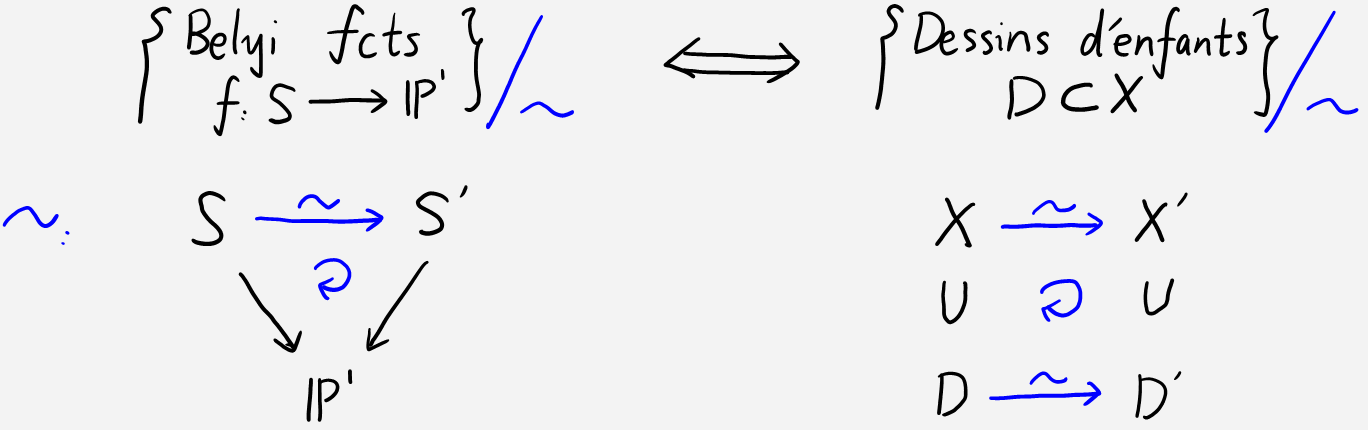
\includegraphics[width=0.8\textwidth]{figures/equivalence.png}
		\end{center}
	\end{proposition}
\end{frame}
\begin{frame}{Example: $S=X=\mathbb{P}^1$}
%	\begin{itemize}
%		\item $f\,(z)=z^n$
%		\item $\displaystyle f\,(z)=-\frac{256}{27}z^3(z-1)$
%		\item $\displaystyle f\,(z)=\frac{3+i}{5}z^3(z-1)^2 \left(z-\frac{4}{25}(4+3i) \right)$
%		\item $\displaystyle f\,(z)=\frac{4}{27} \frac{(1-z+z^2)^3}{z^2(z-1)^2}$
%%		\item $\displaystyle f(z)=C\frac{z^4 (z-1)^2}{z-\frac{11+2\sqrt{10}}{18}}$.
%	\end{itemize}
\begin{figure}[th]
	\begin{minipage}[b]{\textwidth}
		\centering
		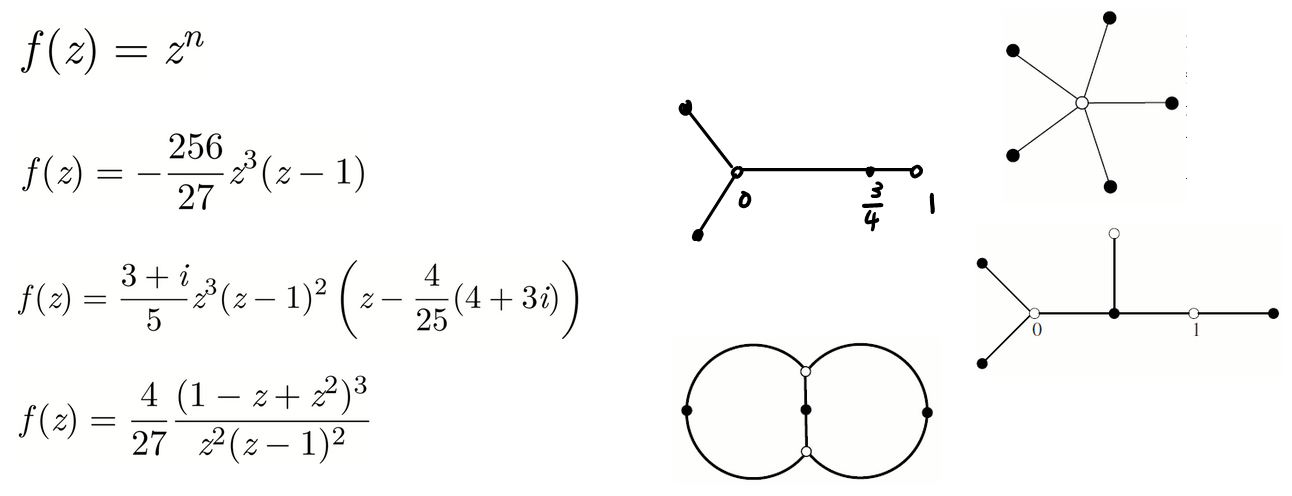
\includegraphics[width=1.05\textwidth]{figures/onepage.png}
	\end{minipage}
\end{figure}
\end{frame}
\begin{frame}{Example: $S=X=\mathbb{P}^1$}
Which one is which?
\begin{figure}[th]
	\begin{minipage}[b]{.2\textwidth}
		\centering
		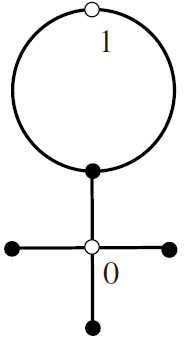
\includegraphics[width=.8\textwidth]{figures/Fig4-32-1.png}
	\end{minipage}
	\begin{minipage}[b]{.2\textwidth}
	\centering
	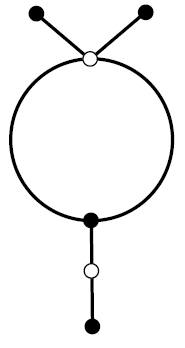
\includegraphics[width=.8\textwidth]{figures/eg6.png}
\end{minipage}
\end{figure}
	 $$\displaystyle f(z)=C\frac{z^4 (z-1)^2}{z-\frac{11+2\sqrt{10}}{18}}\qquad\qquad f(z)=C'\frac{z^4 (z-1)^2}{z-\frac{11-2\sqrt{10}}{18}}$$
\end{frame}
\begin{frame}{Example: $S=X=\mathbb{P}^1$}
\begin{figure}[th]
	\begin{minipage}[b]{.45\textwidth}
		\centering
		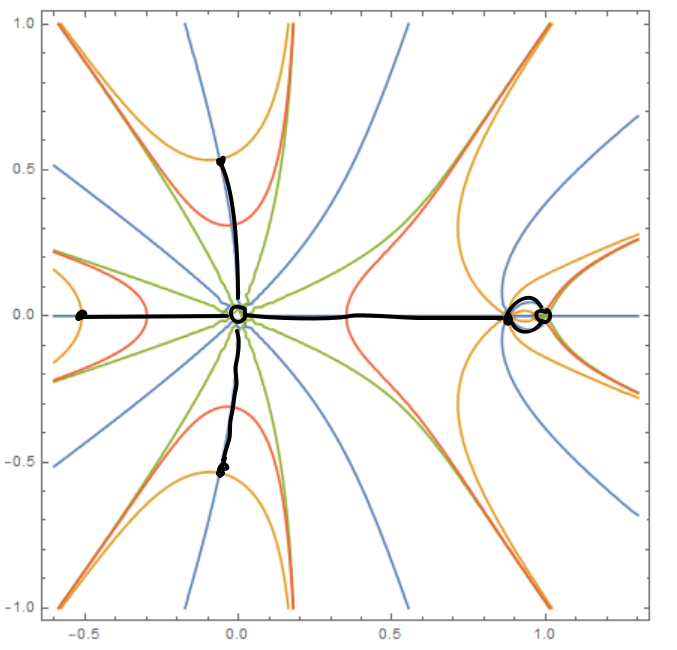
\includegraphics[width=.83\textwidth]{figures/f1=11+2.png}
	\end{minipage}
	\begin{minipage}[b]{.45\textwidth}
		\centering
		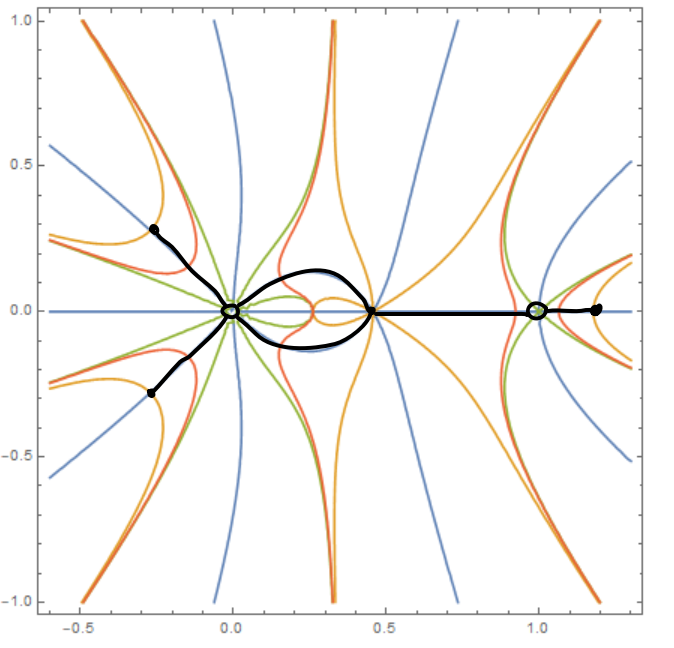
\includegraphics[width=.83\textwidth]{figures/f1=11-2.png}
	\end{minipage}
\end{figure}
$$\displaystyle f(z)=C\frac{z^4 (z-1)^2}{z-\frac{11+2\sqrt{10}}{18}}\qquad\qquad f(z)=C'\frac{z^4 (z-1)^2}{z-\frac{11-2\sqrt{10}}{18}}$$
\end{frame}

\begin{frame}{Proof of Prop 4.20: Step 1}
Given a pair $(X,D)$, we need
	\begin{itemize}
		\item give a RS structure of $X$;
		\item give a fct $f:X\longrightarrow \mathbb{P}^1$.
	\end{itemize}
\begin{figure}[th]
	\begin{minipage}[b]{\textwidth}
		\centering
		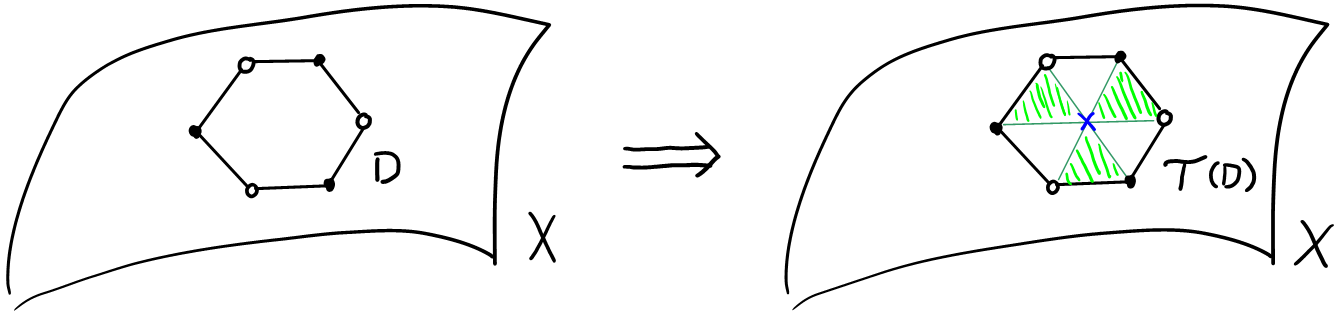
\includegraphics[width=.9\textwidth]{figures/refill.png}
	\end{minipage}
\end{figure}
\vspace{3mm}
\begin{figure}[th]
	\begin{minipage}[t]{.45\textwidth}
		\centering
		\vspace{-1cm}
		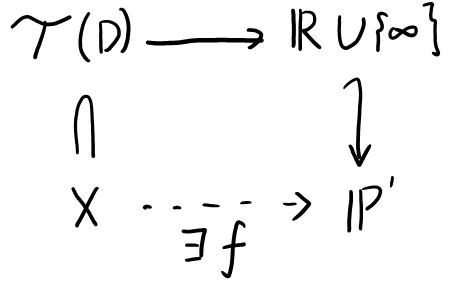
\includegraphics[width=.9\textwidth]{figures/refill2.png}
	\end{minipage}
\hfill
	\begin{minipage}[t]{.45\textwidth}
	$f$ gives a RS structure of X (Riemann compactification) 
\end{minipage}
\end{figure}
\end{frame}
\begin{frame}{Proof of Prop 4.20: Step 2}
\begin{proposition}[Prop 4.20]
	We have an \textbf{equivalence}
	\begin{center}
		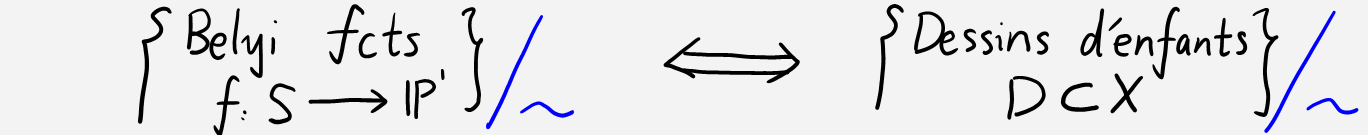
\includegraphics[width=0.8\textwidth]{figures/equivalence2.png}
	\end{center}
	\begin{center}
	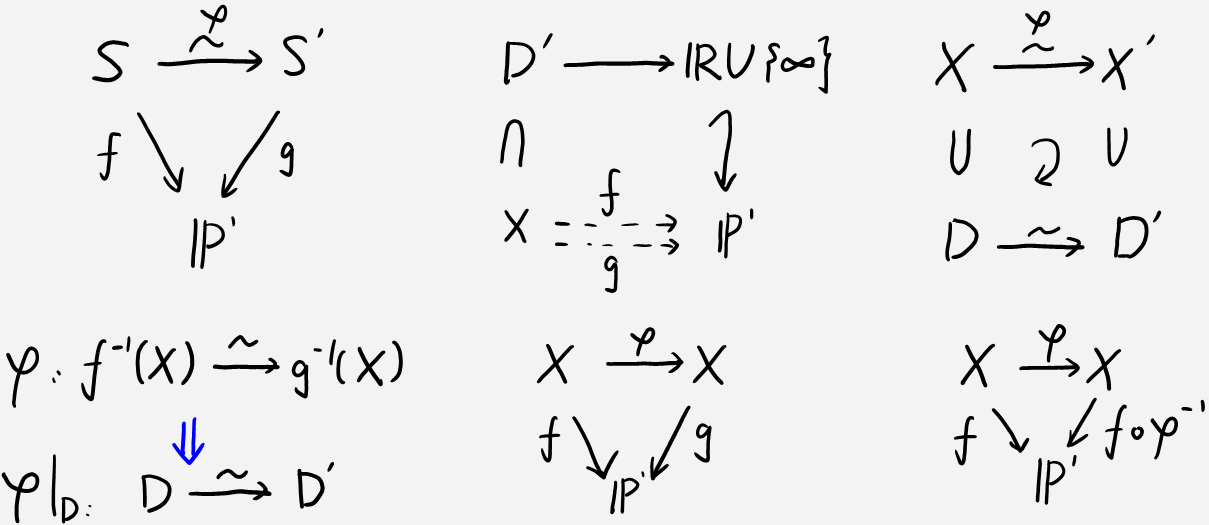
\includegraphics[width=0.8\textwidth]{figures/compatability.png}
\end{center}
\end{proposition}

\end{frame}
\begin{frame}{Proof of Prop 4.20: Step 3}
	$$(X,D) \rightarrow (X_D,f_D) \rightarrow (X_D,D_{f_D}) \qquad (X,D) \sim (X_D,D_{f_D})?$$
	$$(S,f) \rightarrow (S,D_f) \rightarrow (S,f_{D_f}) \qquad (S,f) \sim (S,f_{D_f})?$$
\end{frame}
\begin{frame}
\begin{remark}
	Belyi maps have some kind of rigid: they're decided by dessins (be viewed as \textbf{skeleton} of Belyi fcts)
\end{remark}
\begin{question}
	Even though the equivalence seems natural and trivial, I still have some questions unsolved about this.
\begin{itemize}
	\item Given a Belyi map, can we carry the dessin d'enfant out \textbf{in algorithm}, rather than see with eyes? (For example, write down the polynomial representation)
	\item Given a complex dessin d'enfants defined on $\mathbb{P}^1$, how do we calculate out the \textbf{corresponding rational fuctions}? Is there an algorithm for this?
\end{itemize}
\end{question}
\end{frame}
\begin{frame}[fragile]{What's corresponding Belyi map?}
\begin{figure}[th]
	\begin{minipage}[b]{\textwidth}
		\centering
		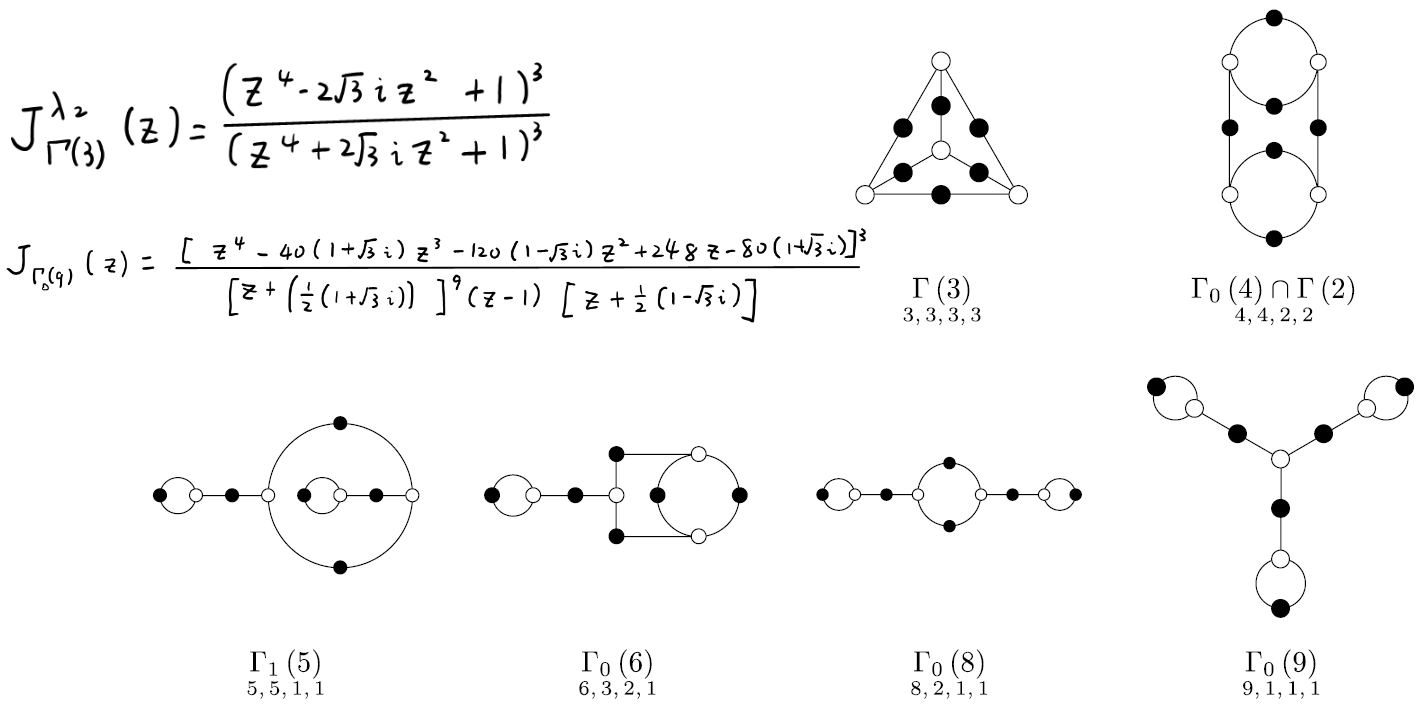
\includegraphics[width=\textwidth]{figures/hardquestion.png}
	\end{minipage}
\end{figure}
\end{frame}


\section{Extract informations from the correspondence}
\subsection{basic information}
\begin{frame}{Contents}
\tableofcontents[currentsection,currentsubsection]
\end{frame}
\begin{frame}[fragile]
		\begin{longtable}{c|c}
		\hline
		$\{\text{Belyi fct}\}/\sim$ & $\{\text{Dessin d'enfants}\}/\sim$	\\
		
		\hline
		\endhead
		\hline
		$\{\text{Belyi fct}\}/\sim$ & $\{\text{Dessin d'enfants}\}/\sim$	\\
		
		\hline
		\endfirsthead	
		\hline
		\endfoot
		\hline		
%		\caption{Correspondence}
		\endlastfoot
		
		$\# f^{-1}(0) + \# f^{-1}(1)$ & $v$\\
		$\# f^{-1}(\infty)$ & $f$ \\
		$\deg f$ & $e$\\
		$2-2g(S)$ & $v+f-e$\\
		Ram index of $x \in f^{-1}(0)$ & $\#$ $\{$black dots adjacent to $x\}$\\
		Ram index of $x \in f^{-1}(1)$ & $\#$ $\{$white dots adjacent to $x\}$\\
		Ram index of $x \in f^{-1}(\infty)$ & $\frac{1}{2}$ $\#$ $\{$sides of face$\}$\\
		
		
		
		\hline								
	\end{longtable}
\end{frame}
\begin{frame}[fragile]
\begin{longtable}{c|c}
	\hline
	$\{\text{Belyi fct}\}/\sim$ & $\{\text{Dessin d'enfants}\}/\sim$	\\
	
	\hline
	\endhead
	\hline
	$\{\text{Belyi fct}\}/\sim$ & $\{\text{Dessin d'enfants}\}/\sim$	\\
	
	\hline
	\endfirsthead	
	\hline
	\endfoot
	\hline		
	%		\caption{Correspondence}
	\endlastfoot
	
	$\# f^{-1}(0) + \# f^{-1}(1)$ & $v$\\
	$\# f^{-1}(\infty)$ & $f$ \\
	$\deg f$ & $e$\\
	$2-2g(S)$ & $v+f-e$\\
	Ram index of $x \in f^{-1}(0)$ & $\#$ $\{$black dots adjacent to $x\}$\\
	Ram index of $x \in f^{-1}(1)$ & $\#$ $\{$white dots adjacent to $x\}$\\
	Ram index of $x \in f^{-1}(\infty)$ & $\frac{1}{2}$ $\#$ $\{$sides of face$\}$\\
	\hline
	monodromy & perm representation pair\\
	"Evenly ramified fct" & uniform dessin\\
	Galois/normal/regular covering & regular dessin\\
	Deck transformation $\Aut (S,f)$ & $\operatorname{Homeo}^+ (X,D)$\\
	\hline
	\multicolumn{2}{c}{Galois action}\\
	\hline
	\multicolumn{2}{c}{construct new from old}\\	
	\hline								
\end{longtable}
\end{frame}
\subsection{monodromy}
\begin{frame}{Contents}
\tableofcontents[currentsection,currentsubsection]
\end{frame}
\begin{frame}{Recall: the monodromy of covering}
\begin{proposition}
		For a covering map $\pi \colon E \longrightarrow B$ and $b_0 \in B$, we have an action
	$$\rho:= \pi_1(B,b_0)^{op} \longrightarrow \Aut (\pi^{-1}(b_0))$$
	which is \textbf{transitive}. We call $Mon(\pi):= \Img \rho$ \textbf{the monodromy group}.
\end{proposition}
	\begin{center}
	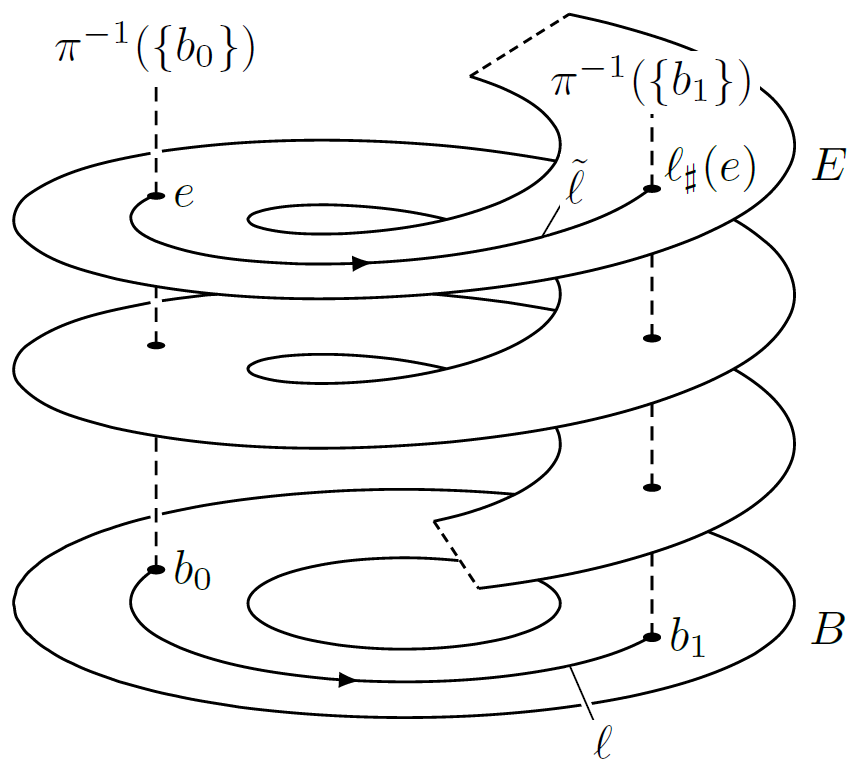
\includegraphics[height=.42\textheight]{figures/coveringlift.png}
\end{center}
\end{frame}
\begin{frame}{Recall: the monodromy of covering}
\begin{proposition}
	For a covering map $\pi \colon E \longrightarrow B$ and $b_0 \in B$, we have an action
	$$\rho:= \pi_1(B,b_0)^{op} \longrightarrow \Aut (\pi^{-1}(b_0))$$
	which is \textbf{transitive}. We call $Mon(\pi):= \Img \rho$ \textbf{the monodromy group}.
\end{proposition}
\begin{center}
	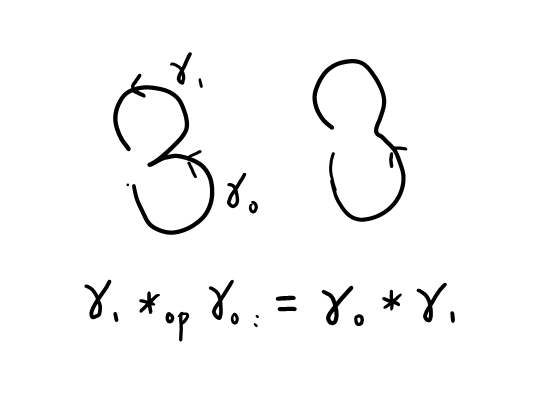
\includegraphics[height=.42\textheight]{figures/op.png}
\end{center}
\end{frame}
\begin{frame}{For Belyi map}
When $B=\mathbb{P}^1 \smallsetminus \{0,1,\infty\}$, then
$\pi_1(B,b_0)=\left\langle\gamma_0,\gamma_1\right\rangle_{free}$.

\begin{center}
	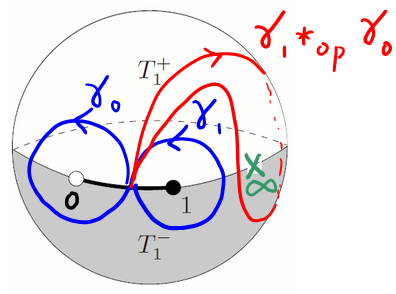
\includegraphics[width=.5\textwidth]{figures/Gamma(2).png}
\end{center}

Denote $\sigma_0:=\rho (\gamma_0), \sigma_1:=\rho (\gamma_1)$, then $Mon(\pi)=\left\langle\sigma_0,\sigma_1\right\rangle$.
\end{frame}
\begin{frame}{For Belyi map}
When $\pi$ is the covering of Belyi map, let $b_0=\frac{1}{2}$, then
\begin{itemize}
	\item $\pi^{-1}(b_0) \longleftrightarrow \{ \text{edges of dessin}\}$
	\item $\sigma_0,\sigma_1$ are permutations of edges, as followed:

\end{itemize}
$(\sigma_0,\sigma_1)$ are called \textbf{the permutation representation pair} of the dessin.
\end{frame}
\begin{frame}[fragile]{$\sigma_0,\sigma_1$}
\begin{figure}[th]
	\begin{minipage}[b]{\textwidth}
		\centering
		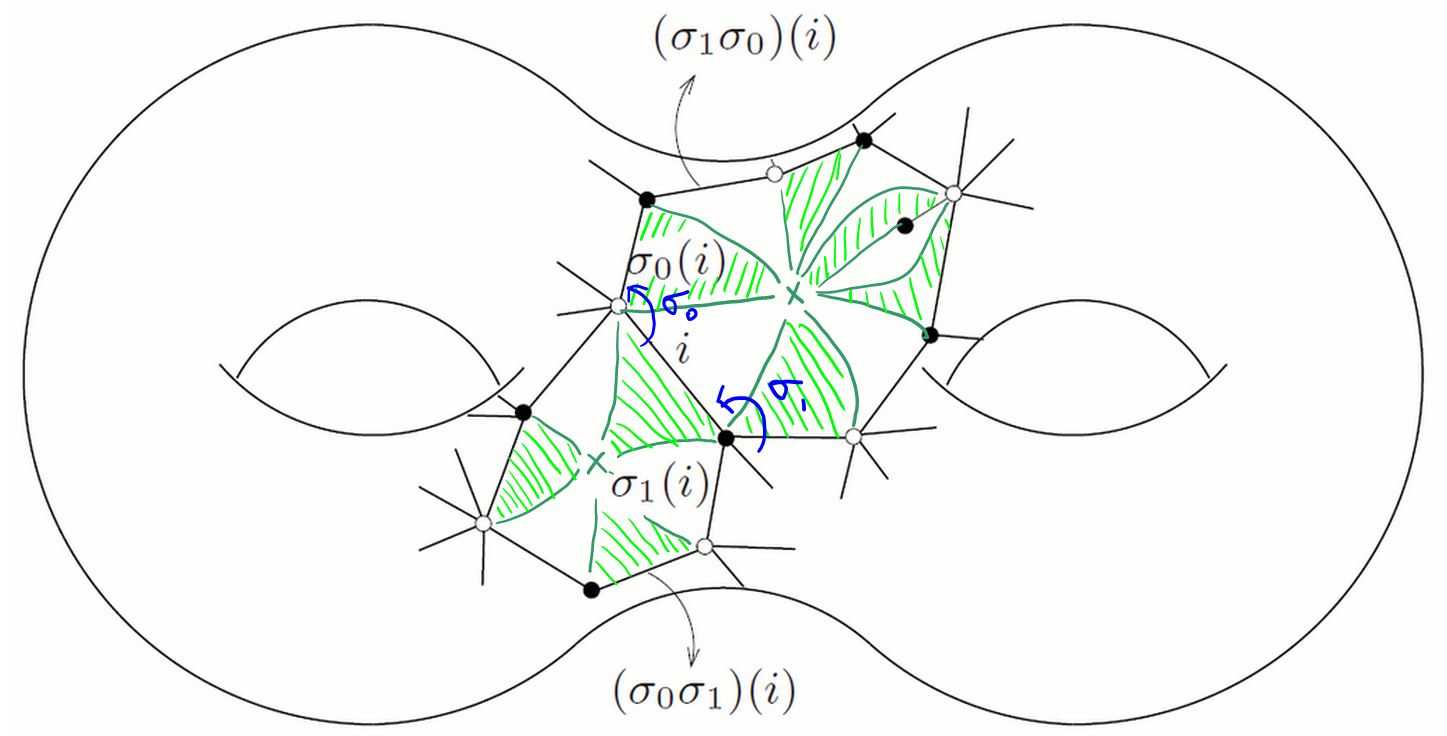
\includegraphics[width=\textwidth]{figures/5.png}
	\end{minipage}
\end{figure}
\end{frame}
\begin{frame}[fragile]{Example: Fig 4.3}
\begin{figure}[th]
	\begin{minipage}[t]{.8\textwidth}
		\centering
		\vspace{0cm}
		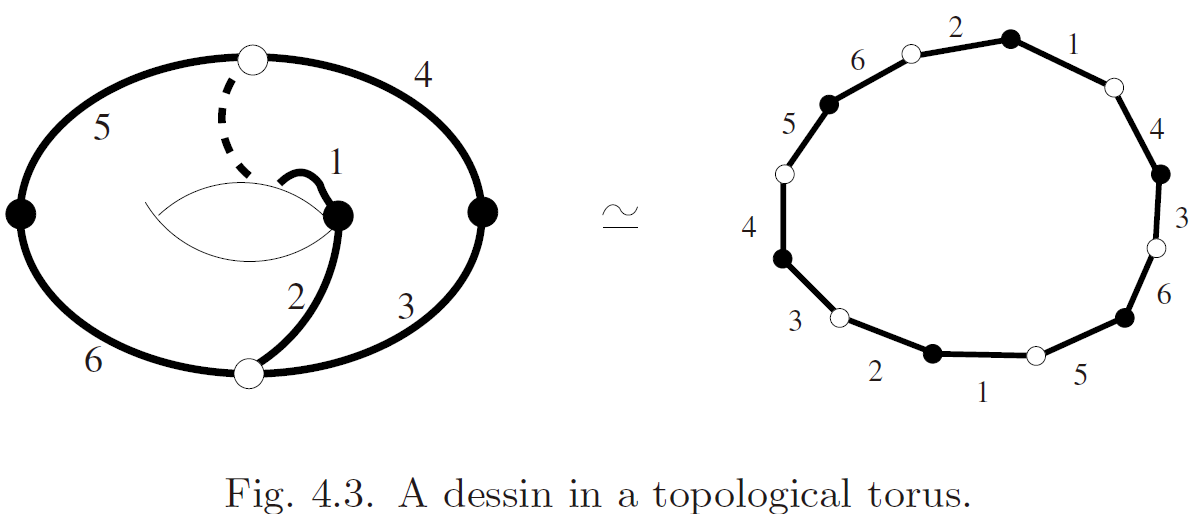
\includegraphics[width=\textwidth]{figures/Fig4-3-2.png}
	\end{minipage}

\begin{minipage}[t]{.4\textwidth}
	\begin{equation*}
		\begin{aligned}
		\sigma_0 & \, = (263)(154) \\
		\sigma_1 & \, = (12)(34)(56) \\
		\sigma_1\sigma_0 & \, = (253164)\\
		\sigma_0\sigma_1 & \, = (253164)
		\end{aligned}
	\end{equation*}
\end{minipage}
\end{figure}
\end{frame}
\begin{frame}[fragile]{Example: Fig 4.3}
\begin{figure}[th]
	\begin{minipage}[t]{.3\textwidth}
		\centering
		\vspace{0cm}
		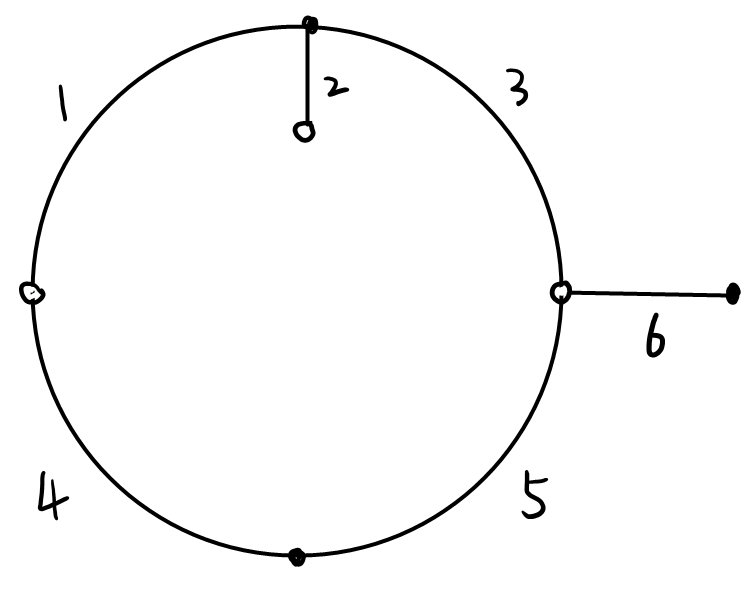
\includegraphics[width=\textwidth]{figures/permrep2.png}
	\end{minipage}
	
	\begin{minipage}[t]{.4\textwidth}
		\begin{equation*}
		\begin{aligned}
		\sigma_0 & \, = (14)(2)(356) \\
		\sigma_1 & \, = (123)(45)(6) \\
		\sigma_1\sigma_0 & \, = (156)(234)\\
		\sigma_0\sigma_1 & \, = (125)(346)
		\end{aligned}
		\end{equation*}
	\end{minipage}
\end{figure}
\end{frame}
%\begin{frame}{Correspondence}
%	\begin{remark}
%		$$\{(X,D)\}/_{\sim} \longleftrightarrow \{  (\sigma_0,\sigma_1) \in \Sigma_N \}/_{\text{conj}}$$
%	\end{remark}
%{
%	\footnotesize
%	% Adjust margins
%	\setlength\LTleft{-0.5in}
%	\setlength\LTright{-1in plus 1 fill}
%	\setlength{\tabcolsep}{4pt}
%\begin{longtable}{c|c|c}
%	\hline
%	$\{\text{Belyi fct}\}/\sim$ & $\{\text{Dessin d'enfants}\}/\sim$	& $\{\text{perm rep pair}\}/\sim $\\
%	
%	\hline
%	\endhead
%	\hline
%	$\{\text{Belyi fct}\}/\sim$ & $\{\text{Dessin d'enfants}\}/\sim$	& $\{\text{perm rep pair}\}/\sim $\\
%	
%	\hline
%	\endfirsthead	
%	\hline
%	\endfoot
%	\hline		
%	%		\caption{Correspondence}
%	\endlastfoot
%	
%	$\# f^{-1}(0) $ & $\#$ $\{$white dots $\}$ &$\#$ $\{$ cycles of  $\sigma_0\}$\\
%	$ \# f^{-1}(1)  $ & $\#$ $\{$black dots $\}$&$\#$ $\{$ cycles of  $\sigma_1\}$\\
%	$\# f^{-1}(\infty)$ & $f$ &$\#$ $\{$ cycles of  $\sigma_1\sigma_0\}$\\
%	$\deg f$ & $e$ & $N=\#$ $\{$ cycles of  $Id\}$\\
%	$2-2g(S)$ & $v+f-e$ & $\#\{\ldots \sigma_0\}$+$\#\{\ldots \sigma_1\}$+$\#\{\ldots \sigma_1\sigma_0\}$-N\\
%	Ram index of $x \in f^{-1}(0)$ & $\#$ $\{$black dots adjacent to $x\}$ & length of a cycle on $\sigma_0$\\
%	Ram index of $x \in f^{-1}(1)$ & $\#$ $\{$white dots adjacent to $x\}$ & length of a cycle on $\sigma_1$\\
%	Ram index of $x \in f^{-1}(\infty)$ & $\frac{1}{2}$ $\#$ $\{$sides of face$\}$ & length of a cycle on $\sigma_0\sigma_1$\\
%	\hline
%								
%\end{longtable}
%}
%\end{frame}
\begin{frame}[fragile]{Correspondence}
	\begin{remark}
	$$\{(X,D)\}/_{\sim} \longleftrightarrow \{  (\sigma_0,\sigma_1) \in \Sigma_N \}/_{\text{conj}}$$
\end{remark}
\begin{figure}[th]
	\begin{minipage}[b]{\textwidth}
		\centering
		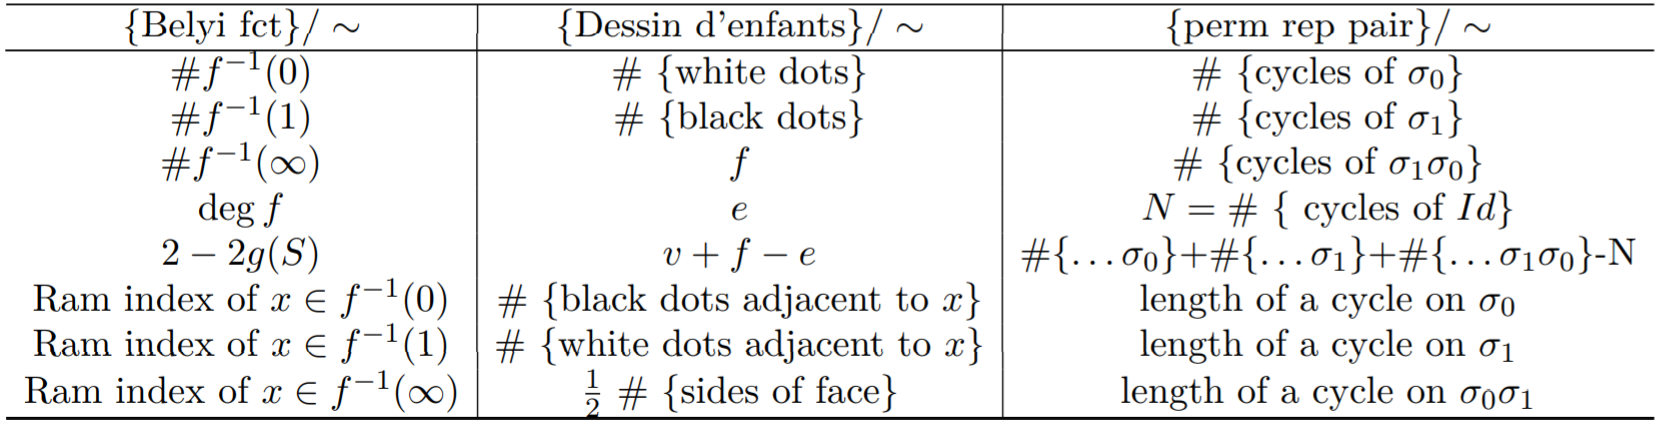
\includegraphics[width=1\textwidth]{figures/table.png}
	\end{minipage}
\end{figure}

\end{frame}
\end{document}




